\documentclass[12pt, a4paper]{article}

\usepackage[utf8]{inputenc}
\usepackage[T1]{fontenc}
\usepackage[italian]{babel}
\usepackage{amsmath, amssymb}
\usepackage{graphicx}
\usepackage{hyperref}
\usepackage{geometry}
\usepackage{booktabs}
\usepackage{caption}
\usepackage{subcaption}
\usepackage{xcolor}
\usepackage{listings}
\usepackage[section]{placeins}

\geometry{margin=2.5cm}
\graphicspath{{Codice/M1_SIR/}{Codice/M2_MCMC/}{Codice/M0_Aux/}}

% Stile per codice MATLAB
\lstdefinestyle{matlab}{
    language=Matlab,
    basicstyle=\ttfamily\small,
    keywordstyle=\color{blue},
    commentstyle=\color{gray}\itshape,
    stringstyle=\color{orange!80!black},
    numbers=left,
    numberstyle=\tiny\color{gray},
    numbersep=8pt,
    breaklines=true,
    frame=single,
    captionpos=b,
    tabsize=4
}

\hypersetup{
    colorlinks=true,
    linkcolor=blue!70!black,
    citecolor=blue!70!black,
    urlcolor=blue!70!black
}

\title{\textbf{Calcolo dell'$R_t$ per l'epidemia\\di COVID-19 in Italia}\\[0.4em]
       \large Due metodi a confronto: modello SIR e simulazione Monte Carlo}
\author{Samuel Seligardi}
\date{Marzo 2026}

\begin{document}

\maketitle

\begin{abstract}
Viene presentato il calcolo dell'indice di riproduzione effettivo $R_t$ per l'epidemia di COVID-19
in Italia nel periodo febbraio~2020 -- gennaio~2025, implementato in MATLAB.
Si confrontano due approcci distinti: un metodo analitico basato sul modello compartimentale SIR,
e un metodo stocastico Monte Carlo di tipo Metropolis ispirato alla metodologia ufficiale
dell'Istituto Superiore di Sanità (ISS).
Il metodo SIR utilizza i dati della Protezione Civile (DPC) -- \texttt{totale\_positivi} come
proxy diretto di $I(t)$ -- ed è parametrizzato con il tempo di rimozione $T_R = 1/\gamma$
specifico di ogni variante circolante; le bande di incertezza riflettono l'errore su $T_R$.
Il metodo Monte Carlo stima $R_t$ massimizzando la verosimiglianza poissoniana tramite
l'algoritmo di Metropolis.
I risultati del metodo SIR vengono confrontati con il dato ufficiale INFN (CovidStat)
disponibile per il periodo 18~marzo~2020 -- 30~marzo~2023.
\end{abstract}

\newpage
\tableofcontents
\newpage

% -------------------------------------------------------
\section{Introduzione}
% -------------------------------------------------------

L'indice di riproduzione effettivo $R_t$ misura il numero medio di nuovi contagi generati da un
individuo infetto al tempo $t$, tenendo conto delle misure di contenimento vigenti e dello stato
immunitario della popolazione.
Un valore $R_t > 1$ indica crescita epidemica; $R_t < 1$ segnala la fase di recessione.
Il monitoraggio in tempo reale di $R_t$ è stato uno degli strumenti centrali della gestione
della pandemia di COVID-19 in Italia.

In questo lavoro si implementano e si confrontano due metodi di calcolo:

\begin{itemize}
    \item \textbf{Metodo SIR} (Sezione~\ref{sec:sir}): ricava $R_t$ in forma chiusa dal modello
          compartimentale SIR.
          Richiede la conoscenza del tempo di rimozione $T_R$, che varia con la variante circolante;
          l'incertezza su $T_R$ viene propagata in bande di errore sul grafico.
          Sono implementate tre varianti che differiscono per la sorgente dati e per l'ordine
          dello smoothing rispetto al calcolo.
    \item \textbf{Metodo Monte Carlo--Metropolis} (Sezione~\ref{sec:mc}): stima $R_t$ giorno per giorno
          massimizzando la verosimiglianza poissoniana tramite un campionamento MCMC, usando
          la distribuzione dei tempi di generazione della letteratura.
          Più accurato ma computazionalmente più costoso.
\end{itemize}

I dati di input sono tre serie storiche pubbliche, descritte in dettaglio
nella Sezione~\ref{sub:dati}:
\begin{itemize}
    \item \texttt{iss-covid19.csv} — nuovi casi ISS per data di prelievo/diagnosi
          (29~gen~2020 -- 6~gen~2026)~\cite{ISS_opendata};
    \item \texttt{dpc-covid19.json} — serie Protezione Civile~\cite{DPC_github}
          con \texttt{nuovi\_positivi} e \texttt{totale\_positivi} per data di referto
          (24~feb~2020 -- 8~gen~2025);
    \item \texttt{infn-rt.csv} — $R_t$ ufficiale INFN CovidStat~\cite{INFN_rt}
          con IC~95\% (18~mar~2020 -- 30~mar~2023).
\end{itemize}

% -------------------------------------------------------
\section{Calcolo basato sul modello SIR}
\label{sec:sir}
% -------------------------------------------------------

\subsection{Il modello SIR}

Il modello compartimentale SIR divide la popolazione (costante $N$) in tre comparti:
suscettibili~$S$, infetti~$I$, rimossi~$R$ (guariti o deceduti).
Il sistema di equazioni differenziali ordinarie è:
\begin{align}
    \frac{d}{dt}S(t) &= -\frac{\beta \, c}{N}\, S(t)\, I(t), \label{eq:dS}\\[4pt]
    \frac{d}{dt}I(t) &= \phantom{-}\frac{\beta \, c}{N}\, S(t)\, I(t) - \gamma\, I(t), \label{eq:dI}\\[4pt]
    \frac{d}{dt}R(t) &= \phantom{-}\gamma\, I(t), \label{eq:dR}
\end{align}
dove $c$ è il numero medio di contatti per persona per unità di tempo, $\beta$ è la probabilità di
trasmissione per contatto, e $\gamma = 1/T_R$ è il tasso di rimozione.
Il numero di riproduzione di base è $R_0 = \beta c / \gamma$.

\subsection{Derivazione della formula operativa}
\label{sub:derivazione}

Sotto l'ipotesi $S(t)/N \approx 1$ (popolazione quasi interamente suscettibile)
e usando la definizione $R_t = (\beta c/\gamma)\,S(t)/N$, dall'equazione~\eqref{eq:dI} si ottiene:
\begin{equation}
    \frac{d}{dt}I(t) = \gamma\,(R_t - 1)\,I(t).
    \label{eq:I_growth}
\end{equation}
Il tasso di crescita relativo degli infetti è quindi proporzionale a $R_t - 1$.
In forma discreta, approssimando la derivata con la differenza all'indietro:
\begin{equation}
    \frac{I(t) - I(t-1)}{I(t)} \approx \gamma\,(R_t - 1) = \frac{R_t - 1}{T_R},
\end{equation}
da cui si ricava la formula operativa:
\begin{equation}
    \boxed{R_t(t) \;=\; 1 + T_R\,\frac{I(t) - I(t-1)}{I(t)}.}
    \label{eq:rt_base}
\end{equation}
Se $I(t)$ viene approssimato dalla somma scorrevole dei nuovi casi negli ultimi $\text{win} = \text{round}(T_R)$
giorni, la variazione si riduce per cancellazione telescopica a soli due termini:
$I(t) - I(t-1) = C(t) - C(t-\text{win})$.

\subsection{Sorgente dati e formula operativa}
\label{sub:dati}

\subsubsection*{Approccio adottato: dati DPC}

I risultati presentati in questo report sono ottenuti con i dati della Protezione Civile
(\texttt{dpc-covid19.json}), che riporta per ogni giorno, tra l'altro,
\texttt{nuovi\_positivi} (flusso) e \texttt{totale\_positivi} (stock degli attualmente positivi).
Quest'ultimo corrisponde \emph{direttamente} a $I(t)$ del modello SIR: non serve nessuna
finestra scorrevole per ricostruire gli infetti attivi.

La formula operativa (funzione \texttt{rt\_dpc.m}) è:
\begin{equation}
    I(t) = \texttt{totale\_positivi}(t), \qquad
    R_t^{\text{raw}}(t) = 1 + T_R\,\frac{I(t) - I(t-1)}{I(t)}, \qquad
    R_t(t) = \frac{1}{7}\sum_{k=0}^{6} R_t^{\text{raw}}(t-k).
    \label{eq:rt_dpc}
\end{equation}
Il post-smoothing su $R_t^{\text{raw}}$ elimina l'artefatto settimanale di referto.

\paragraph{Ritardo strutturale.}
I dati DPC usano la \emph{data di referto}, più tarda della data di inizio sintomi
adottata dall'ISS per il calcolo ufficiale di $R_t$.
Questo introduce un ritardo sistematico di circa una settimana tra la stima SIR e il dato INFN.

\subsubsection*{Varianti alternative disponibili nel codice}

L'implementazione supporta anche la sorgente ISS (\texttt{iss-covid19.csv}, data di prelievo),
con due strategie di smoothing selezionabili via flag:

\begin{itemize}
    \item \textbf{Pre-smooth} (\texttt{rt\_iss\_pre.m}): media mobile a 7 giorni su $C(t)$
          prima del calcolo; $I(t)$ ricostruito come somma scorrevole sui $\text{win} = \text{round}(T_R)$
          giorni precedenti.
    \item \textbf{Post-smooth} (\texttt{rt\_iss\_post.m}): $R_t^{\text{raw}}$
          calcolato dai casi grezzi, poi media mobile su $R_t$.
\end{itemize}

Entrambe le varianti ricostruiscono $I(t)$ dalla somma $\sum_{k=0}^{\text{win}-1} C(t-k)$,
necessaria perché il dato ISS non include gli attivi.
Il confronto tra le varianti è possibile cambiando i flag \texttt{DATA\_SOURCE} e
\texttt{SMOOTH\_MODE} in \texttt{main\_sir.m}.

\subsection{Il parametro \texorpdfstring{$T_R$}{TR} per variante}
\label{sub:TR}

Il tempo di rimozione $T_R = 1/\gamma$ si riduce con le varianti più recenti,
che hanno ciclo infettivo più breve.
La Tabella~\ref{tab:TR} riporta i valori adottati nell'implementazione con le relative
incertezze, usate per generare le bande di errore sui grafici.

\begin{table}[htbp]
\centering
\caption{Parametro $T_R$ per fase epidemica e relativa incertezza.}
\label{tab:TR}
\begin{tabular}{llccc}
\toprule
\textbf{Fase} & \textbf{Variante} & \textbf{Periodo} & $T_R$ \textbf{(giorni)} & $\Delta T_R$ \\
\midrule
1 & Ancestrale + Alpha & feb~2020 -- lug~2021 & $9{,}7$ & $\pm 2{,}0$ \\
2 & Delta              & lug~2021 -- dic~2021 & $7{,}0$ & $\pm 1{,}0$ \\
3 & Omicron BA.1/BA.2  & gen~2022 -- mag~2022 & $6{,}0$ & $\pm 1{,}0$ \\
4 & Omicron BA.5+      & giu~2022 -- mar~2023 & $5{,}0$ & $\pm 1{,}0$ \\
5 & Post-INFN (XBB+)   & apr~2023 -- gen~2025 & $5{,}0$ & $\pm 1{,}0$ \\
\bottomrule
\end{tabular}
\end{table}

\noindent
Il valore $T_R = 9{,}7 \pm 2{,}0$ giorni è ottenuto fittando le equazioni SIR ai dati della
seconda e terza ondata italiana~\cite{Lazzizzera2021}.
Per le varianti successive si adotta uno scaling proporzionale al tempo di generazione:
\begin{equation}
    T_R(\text{var}) \;=\; 9{,}7 \times \frac{\overline{GT}(\text{var})}{\overline{GT}(\text{anc})},
    \label{eq:TR_scaling}
\end{equation}
dove $\overline{GT}$ è il \emph{realized generation time} medio da una meta-analisi
sistematica di 280 studi~\cite{Xu2023}: 4{,}95 giorni (ancestrale), 3{,}65 (Delta),
2{,}99 (BA.1/BA.2).
Per BA.5+ il GT non è disponibile in~\cite{Xu2023}; si usa il serial interval
$SI = 2{,}37$ giorni, grandezza analoga ma non identica al GT (può essere negativo
in presenza di trasmissione presintomatica).
I valori di $\overline{GT}$ per Delta e Omicron sono coerenti con la stima indipendente
di~\cite{Park2023} (3{,}8 e 3{,}0 giorni rispettivamente).

La formula~\eqref{eq:TR_scaling} si basa sull'ipotesi che il rapporto $T_R/\overline{GT}$
sia costante tra varianti, ovvero che la struttura temporale della trasmissione
(in quale momento del periodo infettivo avvengono i nuovi contagi) non cambi al cambiare
della variante.
È opportuno sottolineare che le stime di $\overline{GT}$ di~\cite{Xu2023}
e~\cite{Park2023} provengono da meta-analisi internazionali, non specifiche per l'Italia:
l'unico parametro calibrato direttamente su dati italiani è $T_R = 9{,}7$ giorni
della Fase~1~\cite{Lazzizzera2021}.
Le differenze tra paesi in demografia, politica vaccinale e comportamento sociale
introducono un'incertezza aggiuntiva, parzialmente catturata nelle bande $\pm\Delta T_R$.

Dalla formula~\eqref{eq:TR_scaling} si ottengono $T_R \approx 7{,}1$, $5{,}9$ e $4{,}6$ giorni,
arrotondati ai valori di Tabella~\ref{tab:TR}.
Il valore per BA.1/BA.2 è coerente con la stima diretta del periodo infettivo
di~\cite[p.~34]{UKHSA2024} (5--7 giorni) e con la misurazione virologica di~\cite{Keske2023}
(shedding infettivo in coltura: 52\% positivi al giorno~7, 13{,}5\% al giorno~10),
fornendo una validazione indipendente dello scaling per questa fase.

Poiché $R_t$ dipende \emph{linearmente} da $T_R$ nella formula~\eqref{eq:rt_dpc},
l'incertezza su $T_R$ si propaga direttamente come incertezza su $R_t$.
In particolare, applicare $T_R = 10$ giorni ai dati Omicron comporta una sovrastima sistematica
di $R_t$ che cresce con $R_t$, fino al 60\% ai picchi di ondata; la Fase 1 è l'unica per cui $T_R = 9{,}7$ è calibrato sui dati italiani.
Va inoltre notato che con Omicron l'assunzione $S/N \approx 1$ del modello SIR inizia a essere
violata (immunità acquisita da vaccinazione e infezione precedente), il che introduce un ulteriore
errore sistematico di natura strutturale.

\subsection{Implementazione MATLAB}

L'implementazione è suddivisa in sei funzioni più uno script principale:

\begin{description}
    \item[\texttt{carica\_dati.m}] Carica la serie dei casi (ISS o DPC) e il riferimento
        INFN con la banda IC~95\%.

    \item[\texttt{definisci\_fasi.m}] Definisce le 5 fasi epidemiche con i rispettivi
        parametri $T_R$, $\Delta T_R$ e attributi grafici.

    \item[\texttt{rt\_dpc.m}] Calcola $R_t$ usando \texttt{totale\_positivi} come $I(t)$
        diretto (formula~\eqref{eq:rt_dpc}). Funzione usata per i risultati presentati.

    \item[\texttt{rt\_iss\_pre.m}, \texttt{rt\_iss\_post.m}]
        Varianti per sorgente ISS: ricostruiscono $I(t)$ dalla somma scorrevole dei nuovi
        casi, rispettivamente con smoothing applicato prima o dopo il calcolo di $R_t$.

    \item[\texttt{main\_sir.m}] Script principale. Per ogni fase:
        \begin{enumerate}
            \item seleziona i dati con un margine di warmup di 30 giorni;
            \item chiama la funzione di calcolo per $T_R$, $T_R - \Delta T_R$ e
                  $T_R + \Delta T_R$, producendo tre curve (centrale + bande);
            \item sovrappone la curva INFN con la banda IC~95\% (grigio);
            \item calcola e stampa due metriche di errore:
                  $\max|R_t^{\text{SIR\_best}} - R_t^{\text{INFN}}|$ e
                  la distanza massima tra le bande SIR e IC~95\% INFN (0 se si sovrappongono);
            \item salva la figura per fase in PNG.
        \end{enumerate}
        Al termine produce un \emph{grafico combinato} di tutte le fasi (Fig.~\ref{fig:all}).
\end{description}

Il nucleo del calcolo nella variante DPC è il seguente:
\begin{lstlisting}[style=matlab, caption={Estratto da \texttt{rt\_dpc.m}.}]
for t = 2 : n
    I_t     = totale_pos_in(t);
    delta_I = totale_pos_in(t) - totale_pos_in(t - 1);
    if I_t > 0
        Rt_raw(t) = 1 + T_R * delta_I / I_t;
    end
end
Rt = movmean(Rt_raw, [6 0], 'omitnan');
\end{lstlisting}

La semplicità del codice riflette la semplicità del metodo: \texttt{totale\_positivi}
è già $I(t)$, quindi basta calcolare la differenza giornaliera e applicare
la formula~\eqref{eq:rt_dpc}.
Il post-smooth con \texttt{movmean([6\,0])} è causale: usa solo i 7 giorni precedenti
(incluso il corrente), senza introdurre informazione futura.

\subsection{Risultati}

\subsubsection*{Panoramica dei dati grezzi}

La Figura~\ref{fig:casi} mostra l'andamento dei nuovi positivi giornalieri sull'intero
periodo analizzato, a titolo di panoramica del dataset.

\begin{figure}[htbp]
    \centering
    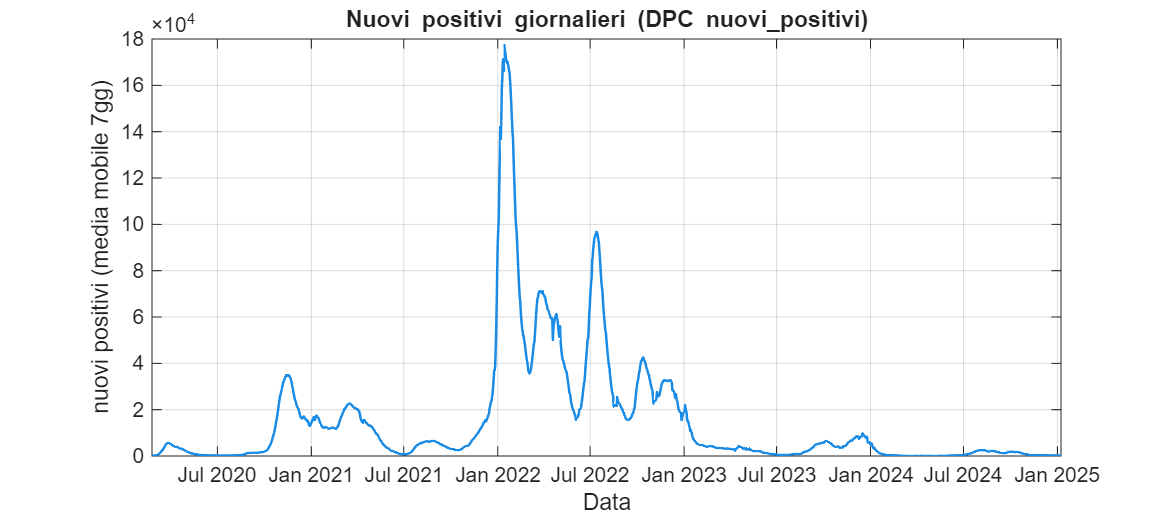
\includegraphics[width=\textwidth]{nuovi_casi.png}
    \caption{Nuovi positivi giornalieri (DPC \texttt{nuovi\_positivi}, media mobile a 7 giorni).
             Le quattro ondate principali corrispondono alle Fasi~1--4.}
    \label{fig:casi}
\end{figure}

\subsubsection*{Andamento per fase}

La Figura~\ref{fig:fase1} e la Figura~\ref{fig:fasi2-5} mostrano $R_t$ calcolato col metodo SIR
(sorgente DPC, formula~\eqref{eq:rt_dpc}) per ogni fase epidemica.
La curva centrale (colorata, piena) usa il valore $T_R$ di Tabella~\ref{tab:TR};
le due curve tratteggiate mostrano $R_t$ calcolato con $T_R \pm \Delta T_R$
e rappresentano la banda di incertezza sul parametro.
In grigio è riportato il valore INFN con l'IC~95\%, dove disponibile.

\begin{figure}[htbp]
    \centering
    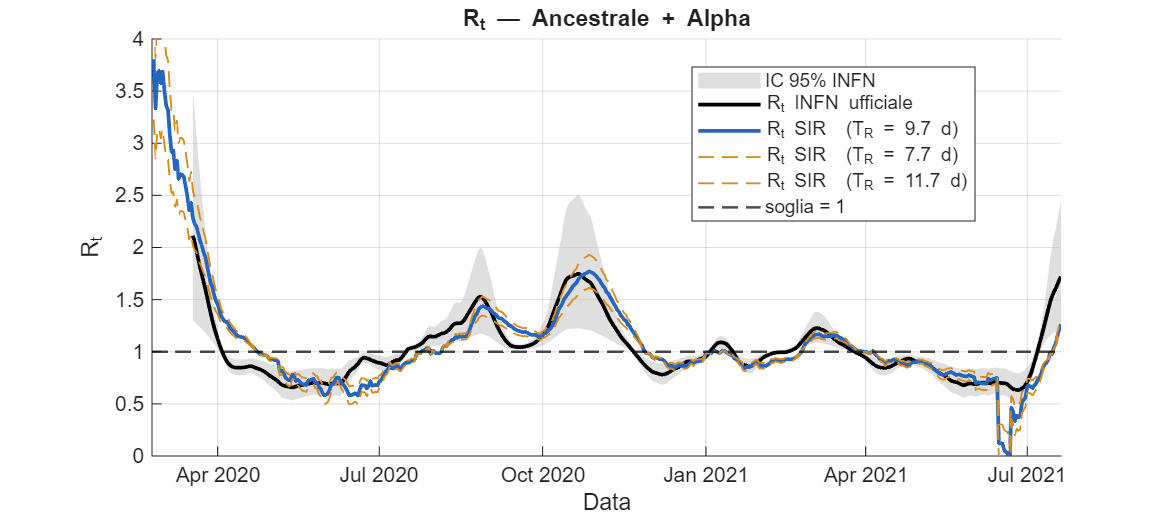
\includegraphics[width=\textwidth]{rt_fase_1_Ancestrale_+_Alpha.png}
    \caption{Fase 1 -- Ancestrale + Alpha (feb~2020 -- lug~2021), $T_R = 9{,}7 \pm 2{,}0$ giorni
             \cite{Lazzizzera2021}.}
    \label{fig:fase1}
\end{figure}

\begin{figure}[htbp]
    \centering
    \begin{subfigure}[b]{0.48\textwidth}
        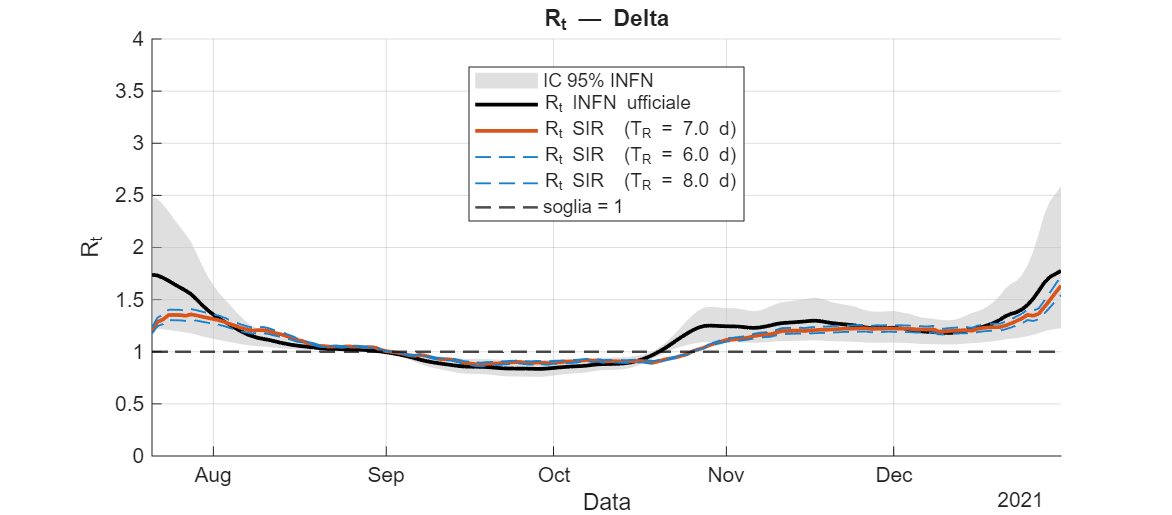
\includegraphics[width=\textwidth]{rt_fase_2_Delta.png}
        \caption{Fase 2 -- Delta, $T_R = 7{,}0 \pm 1{,}0$ d.}
        \label{fig:fase2}
    \end{subfigure}
    \hfill
    \begin{subfigure}[b]{0.48\textwidth}
        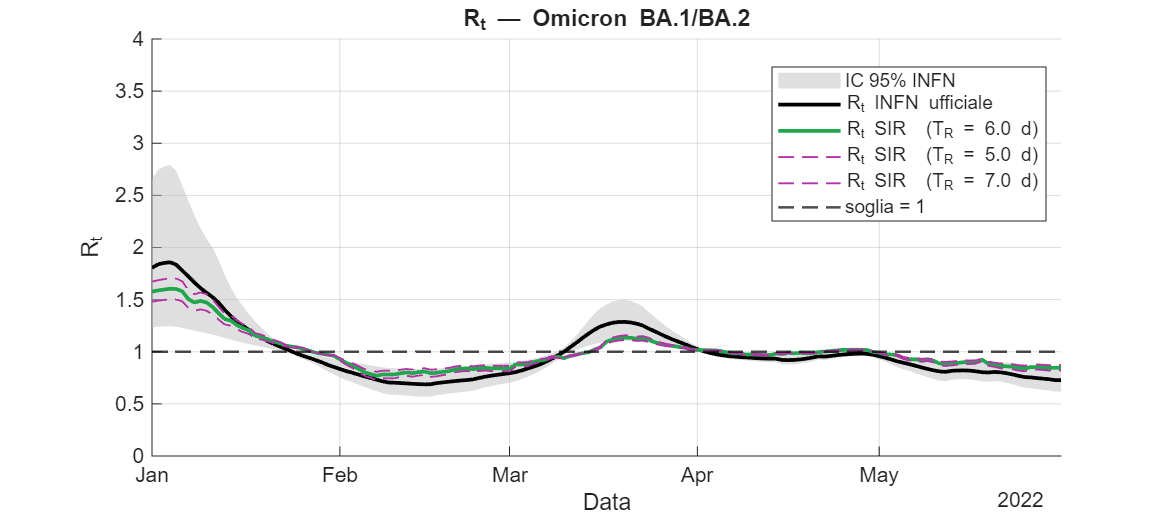
\includegraphics[width=\textwidth]{rt_fase_3_Omicron_BA.1_BA.2.png}
        \caption{Fase 3 -- BA.1/BA.2, $T_R = 6{,}0 \pm 1{,}0$ d.}
        \label{fig:fase3}
    \end{subfigure}

    \vspace{0.5em}

    \begin{subfigure}[b]{0.48\textwidth}
        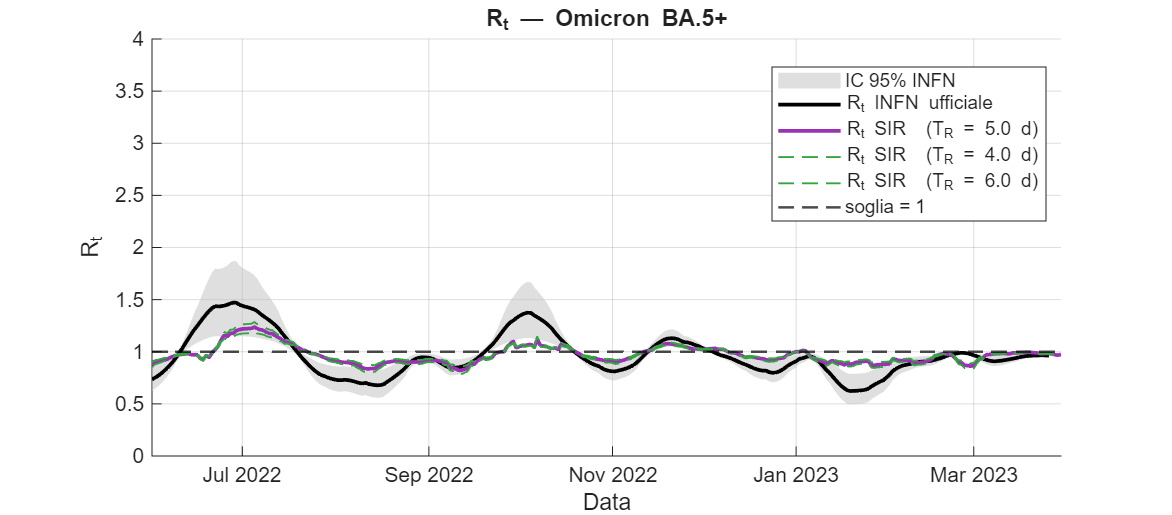
\includegraphics[width=\textwidth]{rt_fase_4_Omicron_BA.5+.png}
        \caption{Fase 4 -- BA.5+, $T_R = 5{,}0 \pm 1{,}0$ d.}
        \label{fig:fase4}
    \end{subfigure}
    \hfill
    \begin{subfigure}[b]{0.48\textwidth}
        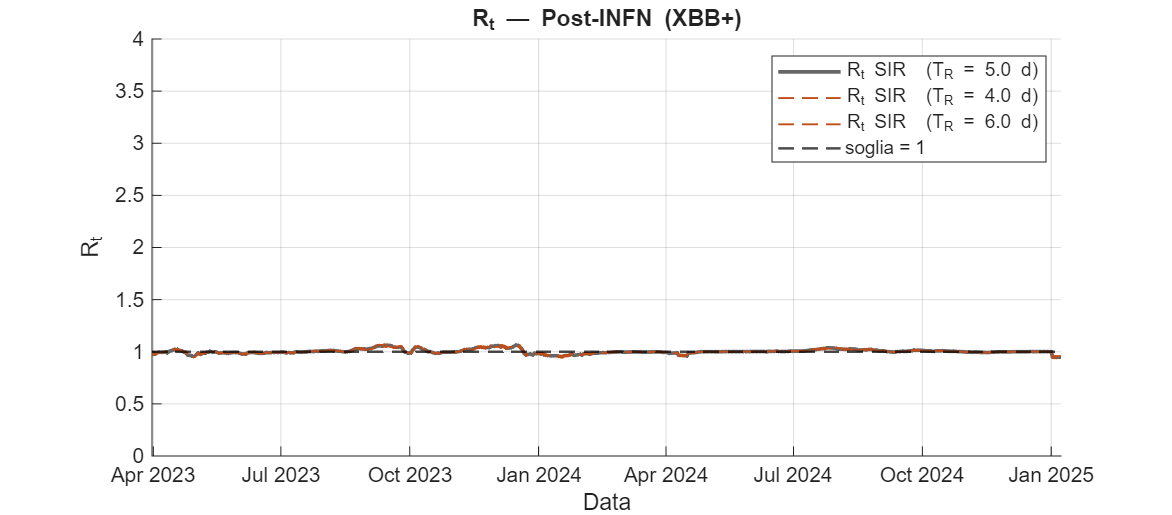
\includegraphics[width=\textwidth]{rt_fase_5_Post-INFN_(XBB+).png}
        \caption{Fase 5 -- XBB+ (nessun dato INFN).}
        \label{fig:fase5}
    \end{subfigure}
    \caption{Fasi 2--5, metodo SIR. Curva SIR colorata, INFN ufficiale in nero,
             IC~95\% in grigio. I valori di $T_R$ sono ottenuti per scaling da
             \cite{Lazzizzera2021} tramite i tempi di generazione di \cite{Xu2023}.}
    \label{fig:fasi2-5}
\end{figure}

\subsubsection*{Andamento complessivo}

La Figura~\ref{fig:all} mostra tutte le fasi concatenate su un asse temporale reale.

\begin{figure}[htbp]
    \centering
    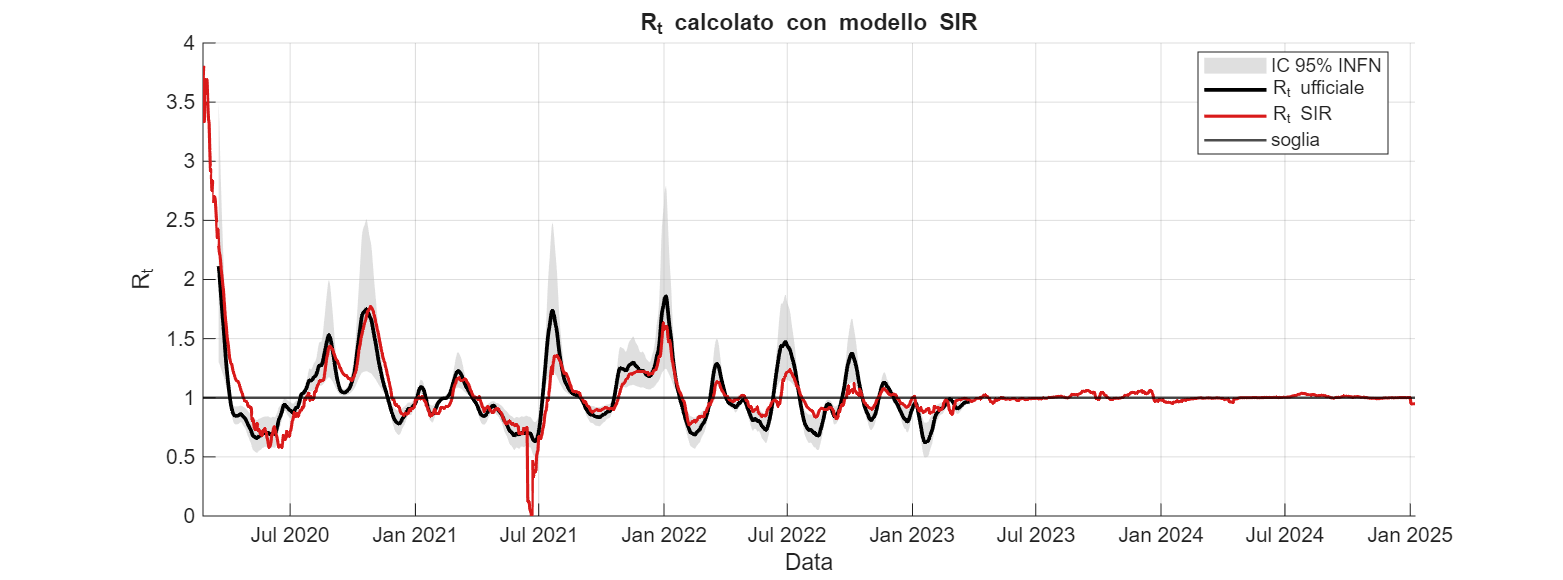
\includegraphics[width=\textwidth]{rt_tutte_le_fasi.png}
    \caption{$R_t$ calcolato con il metodo SIR su tutte le fasi.
             In rosso la curva SIR; in nero la curva INFN ufficiale con banda IC~95\% (grigio).}
    \label{fig:all}
\end{figure}

\subsubsection*{Errori numerici}

La Tabella~\ref{tab:errori_sir} riporta due metriche di errore per ogni fase.

\textbf{Prima colonna} --- per ogni giorno si prende la distanza minima tra le tre curve SIR
(centrale, $T_R - \Delta T_R$, $T_R + \Delta T_R$) e la curva centrale INFN; si riporta
il massimo di questo valore su tutti i giorni della fase.
Risponde alla domanda: scegliendo il $T_R$ ottimale giorno per giorno, qual è il peggior
errore puntuale che si commette?

\textbf{Seconda colonna} --- gap massimo tra la banda SIR $[R_t^{lo},\, R_t^{hi}]$
e la banda IC~95\% INFN $[R_t^{\text{low}},\, R_t^{\text{up}}]$, definito come:
\[
    \max\bigl(0,\; \max(R_t^{lo} - R_t^{\text{up}},\; R_t^{\text{low}} - R_t^{hi})\bigr).
\]
Vale \textbf{0} se le due bande si sovrappongono in ogni giorno della fase,
ed è positivo solo quando sono completamente separate.
Va notato che le due bande rappresentano nature di incertezza diverse: la banda SIR
riflette l'incertezza \emph{parametrica} su $T_R$, mentre l'IC~95\% INFN è
un'incertezza \emph{statistica} sulla stima di $R_t$ dalla likelihood poissoniana.
Il confronto non è quindi formalmente omogeneo e va inteso come un semplice
check di compatibilità visiva, non come un test statistico.
La metrica più interpretabile rimane la prima colonna.

\begin{table}[htbp]
\centering
\caption{Errori metodo SIR vs INFN per fase.}
\label{tab:errori_sir}
\begin{tabular}{llcc}
\toprule
\textbf{Fase} & \textbf{Variante} & \textbf{Max $|R_t^{\text{SIR}} - R_t^{\text{INFN}}|$}
              & \textbf{Max gap bande} \\
\midrule
1 & Ancestrale + Alpha & 0{,}577 & 0{,}454 \\
2 & Delta              & 0{,}507 & 0{,}084 \\
3 & Omicron BA.1/BA.2  & 0{,}193 & 0{,}062 \\
4 & Omicron BA.5+      & 0{,}435 & 0{,}178 \\
\bottomrule
\end{tabular}
\end{table}

\noindent
Il metodo SIR produce una stima in \emph{ritardo} di circa una settimana rispetto al dato
INFN ufficiale, per le ragioni strutturali discusse nella Sezione~\ref{sub:dati}.
L'errore sulla curva centrale (prima colonna) è contenuto nella Fase~3 (0{,}193),
mentre risulta più elevato nelle Fasi~1 e~2 a causa del ritardo temporale strutturale
e nella Fase~4 per la violazione dell'ipotesi $S/N \approx 1$ in fase Omicron avanzata.

Utilizzando la sorgente ISS con post-smoothing (\texttt{rt\_iss\_post.m}), gli errori
scendono a 0{,}292 / 0{,}185 / 0{,}358 nelle Fasi~1, 2 e~4, grazie alla data di prelievo
più vicina alla data di inizio sintomi adottata da INFN.
La Fase~3 costituisce un'eccezione (0{,}432 vs 0{,}193): con Omicron la riduzione massiva
dei tamponi ha reso la serie ISS più rumorosa, rendendo la stima DPC più accurata in
questa fase.

\paragraph{Limite della variante DPC nella Fase~5.}
Nella Fase~5 (apr~2023 -- gen~2025, priva di dato INFN di riferimento) la curva SIR ottenuta con
\texttt{totale\_positivi} DPC risulta artificialmente piatta, con $R_t \approx 1$ costante.
Ciò non riflette la realtà epidemiologica, bensì un degrado del dato: con la fine
dell'emergenza COVID (maggio~2023) il tracciamento sistematico dei positivi è stato
drasticamente ridotto, e lo \emph{stock} \texttt{totale\_positivi} ha smesso di variare
significativamente.
Il \emph{flusso} giornaliero (\texttt{nuovi\_positivi} DPC, o i casi ISS per data di prelievo)
continua invece a oscillare in modo informativo, poiché anche con meno tamponi il segnale
giornaliero preserva la dinamica epidemica.
Le varianti ISS (\texttt{rt\_iss\_pre.m}, \texttt{rt\_iss\_post.m}) e il Metodo~2
(Monte Carlo, che usa \texttt{nuovi\_positivi} DPC) producono una Fase~5 più aderente
alla realtà, confermando che il problema è nella sorgente dati e non nel metodo.

% -------------------------------------------------------
\section{Calcolo con simulazione Monte Carlo}
\label{sec:mc}
% -------------------------------------------------------

\subsection{Distribuzione dei tempi di generazione}

Il metodo Monte Carlo adottato è ispirato alla metodologia ufficiale ISS \cite{Merler2020}
(si veda la Sezione~\ref{sub:epiestim} per le differenze rispetto al metodo ufficiale INFN).
Il punto di partenza è la \emph{distribuzione dei tempi di generazione} $\varphi(s)$, che
descrive la probabilità che un individuo infettato al giorno $t-s$ generi un nuovo caso al
giorno $t$.

Si adotta una distribuzione Gamma con parametri stimati da dati italiani da Cereda et al.~\cite{Cereda2020}
e ripresi da Guzzetta e Merler~\cite{Guzzetta2020}:
\begin{equation}
    \varphi(s) \propto s^{\alpha - 1}\, e^{-s/\theta},
    \qquad \alpha = 1{,}87\;\;(\text{SD}\;0{,}26),\quad
    \beta = 0{,}28\;\;(\text{SD}\;0{,}04),\quad
    \theta = \frac{1}{\beta} \approx 3{,}57 \text{ giorni},
    \label{eq:gamma_dist}
\end{equation}
con valore atteso $\mu = \alpha\theta \approx 6{,}6$ giorni e deviazione standard
$\sigma = \sqrt{\alpha}\,\theta \approx 4{,}9$ giorni.
Questi sono gli stessi parametri adottati dal gruppo INFN CovidStat~\cite{INFN_rt_info}.
La distribuzione è troncata a 25 giorni (il contributo oltre tale soglia è inferiore a
$2 \times 10^{-3}$ e quindi trascurabile).

La discretizzazione viene eseguita tramite integrazione numerica (\texttt{quad} di MATLAB) su
intervalli unitari, non con il valore puntuale della densità:
\begin{equation}
    \varphi_s = \int_{s-0{,}5}^{s+0{,}5} \mathrm{Gamma}(u;\,\alpha,\,\theta)\,du,
    \qquad s = 1, 2, \ldots, 25.
    \label{eq:phi_discrete}
\end{equation}
Dopo la troncatura si rinormalizza: $\varphi_s \leftarrow \varphi_s / \sum_{s=1}^{25} \varphi_s$.

La Figura~\ref{fig:phi} mostra le barre $\varphi_s$ usate nel calcolo confrontate con
la densità Gamma continua.

\begin{figure}[htbp]
    \centering
    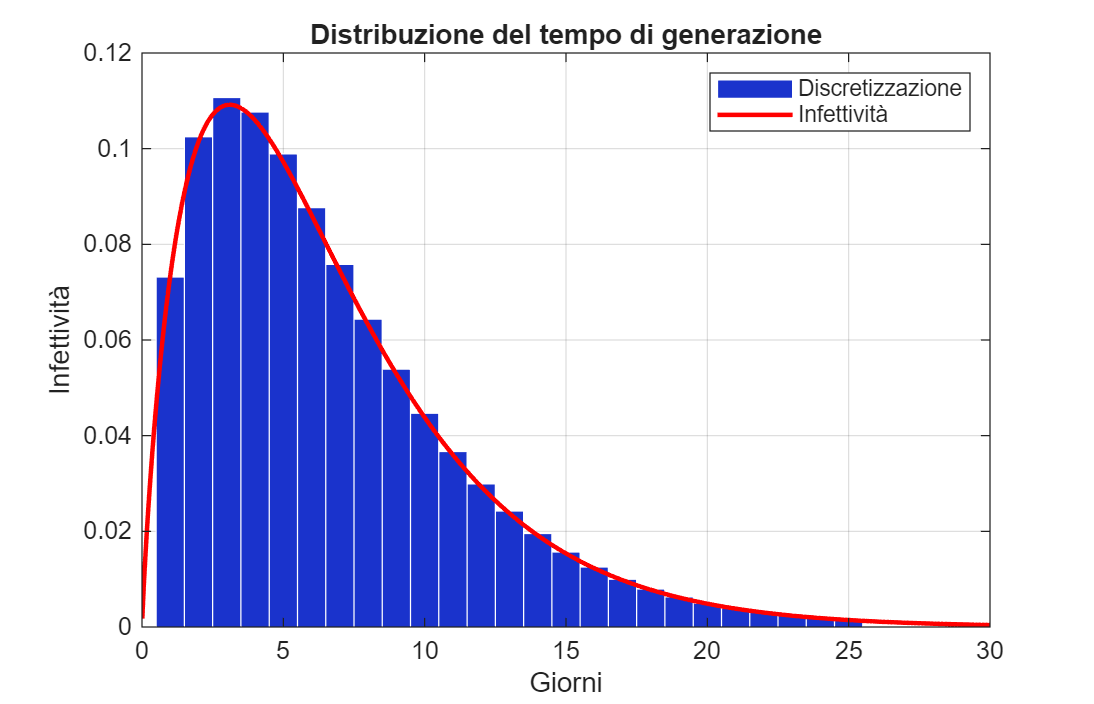
\includegraphics[width=0.75\textwidth]{phi_distribuzione.png}
    \caption{Distribuzione discreta del tempo di generazione $\varphi_s$ (barre blu,
             somma = 1) e densità Gamma continua (curva rossa).
             La troncatura a 25 giorni cattura oltre il 98\% della distribuzione.}
    \label{fig:phi}
\end{figure}

\subsection{Funzione di verosimiglianza}

Il metodo utilizza come input la serie $C(t)$ dei nuovi casi giornalieri.
Nella formulazione originale ISS si usano i soli casi \emph{sintomatici}, circa 100 volte
meno numerosi dei positivi totali ma più robusti perché indipendenti dalla politica di testing;
tale serie non è però disponibile pubblicamente;
nell'implementazione si usa \texttt{nuovi\_positivi} DPC come proxy (si veda la giustificazione a fine sezione).

Il numero atteso di casi al giorno $t$, dato $R_t$, è:
\begin{equation}
    \lambda(t) = R_t\,\lambda_{\text{base}}(t), \qquad
    \lambda_{\text{base}}(t) = \sum_{s=1}^{25} \varphi_s\, C(t-s),
    \label{eq:lambda}
\end{equation}
dove $\lambda_{\text{base}}(t)$ è la forza di infezione attesa al giorno $t$ determinata dai
casi passati, pesati con la distribuzione dei tempi di generazione $\varphi$.
Il modello presuppone che i contagi siano indipendenti condizionatamente a $R_t$, con distribuzione
poissoniana:
\begin{equation}
    P\bigl(C(t)\,\big|\,\lambda(t)\bigr) = \frac{\lambda(t)^{C(t)}\, e^{-\lambda(t)}}{C(t)!}.
    \label{eq:poisson}
\end{equation}
Poiché $R_t$ viene stimato un giorno alla volta in modo indipendente,
la verosimiglianza per il giorno $t$ coincide con la probabilità appena scritta:
$\mathcal{L}(R_t) = P\bigl(C(t)\,\big|\,\lambda(t)\bigr)$.
Prendendo il logaritmo, la log-verosimiglianza del giorno $t$ è:
\begin{equation}
    \ell\bigl(R_t\bigr) = C(t)\ln\lambda(t) - \lambda(t) - \ln\bigl[C(t)!\bigr].
    \label{eq:loglik}
\end{equation}
Poiché $\lambda$ è lineare in $R_t$, la log-verosimiglianza $\ell$ è concava in $R_t$ e il suo
massimo è la stima MLE $\hat{R}_t = C(t)/\lambda_{\text{base}}(t)$.

L'uso di \texttt{nuovi\_positivi} DPC come proxy è giustificato proprio da questa formula:
se $C(t)$ viene moltiplicata per un fattore costante $k$, anche $\lambda_{\text{base}}$
viene moltiplicata per $k$ e il rapporto — quindi $\hat{R}_t$ — rimane invariato.

\subsection{Algoritmo Metropolis}
\label{sub:metropolis}

Per stimare $R_t$ al giorno $t$ si usa l'algoritmo di Metropolis, che esplora lo spazio dei
possibili valori di $R_t$ con un campionamento MCMC.

\begin{enumerate}
    \item \textbf{Inizializzazione:} $R_t^{(0)} = 1$.
    \item \textbf{Proposta:} si estrae un candidato
          $R_t^* = R_t^{(k)} + U(-\delta, +\delta)$, con $\delta = 1{,}5$ fisso
          (proposta uniforme non adattiva).
    \item \textbf{Accettazione:} si calcola il rapporto di verosimiglianza
          \begin{equation}
              \rho = \frac{\mathcal{L}(R_t^*)}{\mathcal{L}(R_t^{(k)})}
                   = \frac{P\bigl(C(t)\,\big|\,\lambda^*\bigr)}{P\bigl(C(t)\,\big|\,\lambda^{(k)}\bigr)}
                   = \frac{e^{\,\ell(R_t^*)}}{e^{\,\ell(R_t^{(k)})}}
                   = \exp\!\bigl[\ell(R_t^*) - \ell(R_t^{(k)})\bigr].
              \label{eq:metropolis_ratio}
          \end{equation}
          Si accetta $R_t^*$ con probabilità $\min(1, \rho)$.
    \item \textbf{Iterazione:} si ripetono i passi 2--3 finché la catena non converge.
\end{enumerate}

\noindent
La verosimiglianza Poisson è unimodale: ha un unico picco in $\hat{R}_t = C(t)/\lambda_{\text{base}}(t)$.
Dopo il burn-in la catena si concentra intorno a quel picco --- i passi che se ne allontanano
vengono rifiutati con alta probabilità --- e la media dei valori post burn-in converge alla media
della distribuzione a posteriori: con prior uniforme quest'ultima è una
$\mathrm{Gamma}\bigl(C(t)+1,\; 1/\lambda_{\text{base}}(t)\bigr)$, la cui media
$\bigl(C(t)+1\bigr)/\lambda_{\text{base}}(t)$ coincide con l'MLE a meno di un fattore relativo
$1/C(t)$.
L'ampiezza fissa $\delta = 1{,}5$ è stata scelta sperimentalmente: valori troppo piccoli rallentano
la convergenza, valori troppo grandi portano a rifiutare quasi ogni proposta.

\paragraph{Proprietà del bilancio dettagliato.}
Il bilancio dettagliato è una condizione \emph{sufficiente} (non necessaria) affinché
$\pi$ sia la distribuzione stazionaria della catena:
\begin{equation}
    \pi(R)\, W(R \to R') = \pi(R')\, W(R' \to R) \qquad \forall\, R, R',
    \label{eq:detailed_balance}
\end{equation}
dove $W(R \to R')$ è la probabilità di transizione e $\pi(R) \propto \mathcal{L}(R_t)$.
Sommando entrambi i membri su $R$:
\[
    \sum_R \pi(R)\,W(R \to R') = \pi(R')\sum_R W(R' \to R) = \pi(R'),
\]
dove l'ultimo passaggio usa $\sum_R W(R' \to R) = 1$ (da ogni stato la catena deve
andare da qualche parte). Il lato sinistro è la probabilità di trovarsi in $R'$
al passo successivo, partendo dalla distribuzione $\pi$: il fatto che sia uguale a
$\pi(R')$ significa che la distribuzione non cambia — ovvero $\pi$ è stazionaria.

\textbf{Derivazione della regola di accettazione.}
Si fattorizza la probabilità di transizione in proposta e accettazione:
\[
    W(R' \to R) = q(R' \to R)\cdot a(R', R),
\]
dove $q$ è la probabilità di proporre il salto e $a \in [0,1]$ quella di accettarlo.
Sostituendo in~\eqref{eq:detailed_balance} e usando la simmetria della proposta
$q(R \to R') = q(R' \to R)$ (proposta uniforme centrata):
\[
    \frac{a(R,\,R')}{a(R',\,R)} = \frac{\pi(R')}{\pi(R)}.
\]
Poiché $a$ dipende solo dal rapporto $\pi(R')/\pi(R)$, scriviamo $a(R,R') = F(z)$
con $z = \pi(R')/\pi(R)$, e analogamente $a(R',R) = F(z^{-1})$.
La condizione $a/a' = z$ diventa allora un vincolo sulla funzione $F$:
\[
    \frac{F(z)}{F(z^{-1})} = z.
\]
La soluzione più semplice è:
\begin{equation}
    F(z) = \min(1,\, z).
    \label{eq:Fmin}
\end{equation}
La regola di accettazione con probabilità $\min(1, \rho)$ — con $\rho = \pi(R^*)/\pi(R^{(k)})$
— non è quindi una scelta arbitraria, ma la conseguenza diretta del bilancio
dettagliato con proposta simmetrica.

\paragraph{Post-processing.}
La serie $R_t$ giornaliera ottenuta viene ulteriormente regolarizzata con una media mobile a 7
giorni, analoga al post-smooth del metodo SIR.

\subsection{Relazione con il metodo ufficiale INFN (EpiEstim)}
\label{sub:epiestim}

Il metodo ufficiale adottato da INFN CovidStat~\cite{INFN_rt_info} e dall'ISS non è il
Metropolis ma \textbf{EpiEstim}~\cite{Cori2013}, sviluppato da Cori et al.\ (2013).
Entrambi i metodi partono dalla stessa equazione di rinnovo~\eqref{eq:lambda} e dalla stessa
verosimiglianza poissoniana~\eqref{eq:poisson}, ma differiscono in due aspetti chiave.

\paragraph{Finestra di stima.}
EpiEstim usa una \emph{finestra scorrevole} di $\tau = 7$ giorni: stima $R_t$ dall'intero
blocco di osservazioni $[t-\tau+1, t]$, non dal solo giorno $t$.
Il metodo Metropolis implementato usa $\tau = 1$ (un singolo giorno per volta), il che
equivale a massimizzare la verosimiglianza puntuale senza lisciamento temporale incorporato.

\paragraph{Metodo di inferenza.}
EpiEstim assume un prior $R_t \sim \mathrm{Gamma}(a, b)$ con $a = b = 5$
(media unitaria, cioè prior centrato su $R_t = 1$).
Poiché la Gamma è coniugata con la Poisson, la distribuzione a posteriori è analitica:
i parametri si aggiornano semplicemente sommando i casi osservati e la forza di infezione
attesa sulla finestra $\tau$:
\begin{equation}
    R_t \,\big|\, \text{dati} \;\sim\; \mathrm{Gamma}\!\left(
        a + \sum_{k=t-\tau+1}^{t} C(k),\;\;
        b + \sum_{k=t-\tau+1}^{t} \lambda_{\text{base}}(k)
    \right),
    \label{eq:epiestim_posterior}
\end{equation}
con media a posteriori $(a + \sum C(k))\,/\,(b + \sum \lambda_{\text{base}}(k))$.
Non è necessario alcun campionamento MCMC.

La Tabella~\ref{tab:confronto_metodi} riassume le principali differenze tra i due approcci.

\begin{table}[htbp]
\centering
\caption{Confronto tra EpiEstim (metodo ufficiale INFN/ISS) e il Metodo Monte Carlo del progetto.}
\label{tab:confronto_metodi}
\begin{tabular}{lll}
\toprule
\textbf{Aspetto}          & \textbf{EpiEstim (INFN/ISS)}            & \textbf{Metropolis (progetto)} \\
\midrule
Finestra di stima         & 7 giorni scorrevoli                     & 1 giorno \\
Posteriore                & Gamma analitica (formula chiusa)        & Campionata con MCMC \\
Prior su $R_t$            & $\mathrm{Gamma}(5,5)$ (configurabile)   & Nessuno (MLE) \\
Implementazione           & R -- pacchetto EpiEstim                 & MATLAB -- da zero \\
\bottomrule
\end{tabular}
\end{table}

Il Metropolis non usa nessun prior: accetta o rifiuta le proposte guardando solo la
verosimiglianza, cercando il valore di $R_t$ che meglio spiega i dati del giorno $t$.
EpiEstim invece incorpora la credenza iniziale $R_t \approx 1$ tramite il prior $\mathrm{Gamma}(5,5)$,
che però diventa trascurabile quando i casi sono abbondanti — nei due metodi le stime convergono.

\subsection{Implementazione MATLAB}

L'implementazione è suddivisa in tre file nella cartella \texttt{M2\_MCMC/}:

\begin{description}
    \item[\texttt{phi\_gamma.m}] Calcola la distribuzione discreta $\varphi_s$ integrando
        numericamente con \texttt{quad} su intervalli $[s-0{,}5,\, s+0{,}5]$.
        La densità Gamma è implementata direttamente con la funzione \texttt{gamma()} built-in,
        senza richiedere la Statistics Toolbox.

    \item[\texttt{metropolis\_rt.m}] Esegue la catena Metropolis per un singolo giorno $t$.
        Riceve in input $C(t)$ e $\lambda_{\text{base}} = \sum_s \varphi_s C(t-s)$
        (già calcolata nel main) e restituisce la media della catena post burn-in.
        Il log-ratio di accettazione si riduce a:
        \begin{equation*}
            \ln\rho = C(t)\ln\!\frac{R_t^*}{R_t} - \lambda_{\text{base}}\,(R_t^* - R_t).
        \end{equation*}

    \item[\texttt{main\_mc.m}] Script principale. Carica i dati tramite
        \texttt{carica\_dati('dpc')}: usa \texttt{nuovi\_positivi} DPC come
        proxy dei casi sintomatici ISS (non disponibili come serie pubblica).
        Calcola $\varphi$ con i parametri $\alpha=1{,}87$, $\theta=1/0{,}28$,
        poi esegue il loop giornaliero:
        \begin{lstlisting}[style=matlab, caption={Nucleo del calcolo in \texttt{main\_mc.m}.}]
for t = S_MAX + 1 : n
    lambda_base = phi' * flipud(casi(t - S_MAX : t - 1));
    Rt_raw(t)   = metropolis_rt(casi(t), lambda_base, ...
                                N_ITER, N_BURNIN, DELTA);
end
Rt_mc = movmean(Rt_raw, [6 0], 'omitnan');
        \end{lstlisting}
        Al termine produce un grafico combinato sull'intero periodo
        e grafici per fase, salvati in \texttt{M2\_MCMC/}.
\end{description}

I parametri Metropolis usati sono: $N_{\text{iter}} = 5000$, $N_{\text{burn-in}} = 500$,
$\delta = 1{,}5$.

\subsection{Risultati}

La Figura~\ref{fig:mc_fase1} e la Figura~\ref{fig:mc_fasi2-5} mostrano $R_t$ calcolato con il metodo
Monte Carlo--Metropolis per tutte le fasi.
Nelle fasi con dato INFN disponibile, la curva MC (colorata) è confrontata con la curva
ufficiale (nera) e la banda IC~95\% (grigio); la Fase~5 è riportata senza riferimento.

\begin{figure}[htbp]
    \centering
    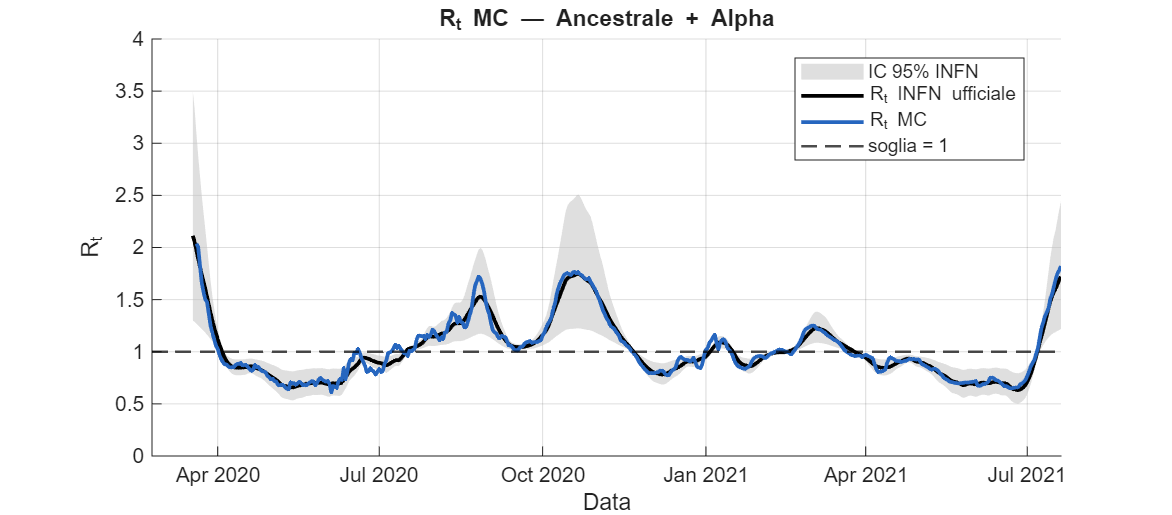
\includegraphics[width=\textwidth]{rt_mc_fase_1_Ancestrale_+_Alpha.png}
    \caption{Fase 1 -- Ancestrale + Alpha (MC Metropolis).}
    \label{fig:mc_fase1}
\end{figure}

\begin{figure}[htbp]
    \centering
    \begin{subfigure}[b]{0.48\textwidth}
        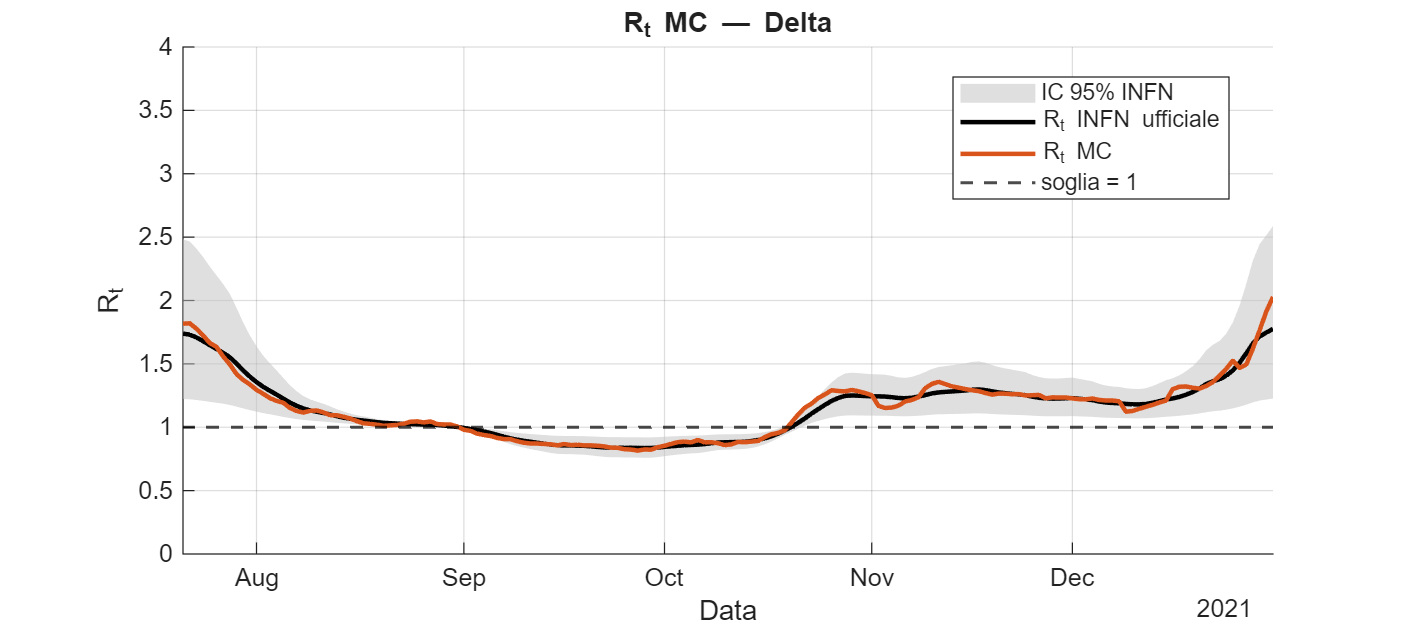
\includegraphics[width=\textwidth]{rt_mc_fase_2_Delta.png}
        \caption{Fase 2 -- Delta.}
        \label{fig:mc_fase2}
    \end{subfigure}
    \hfill
    \begin{subfigure}[b]{0.48\textwidth}
        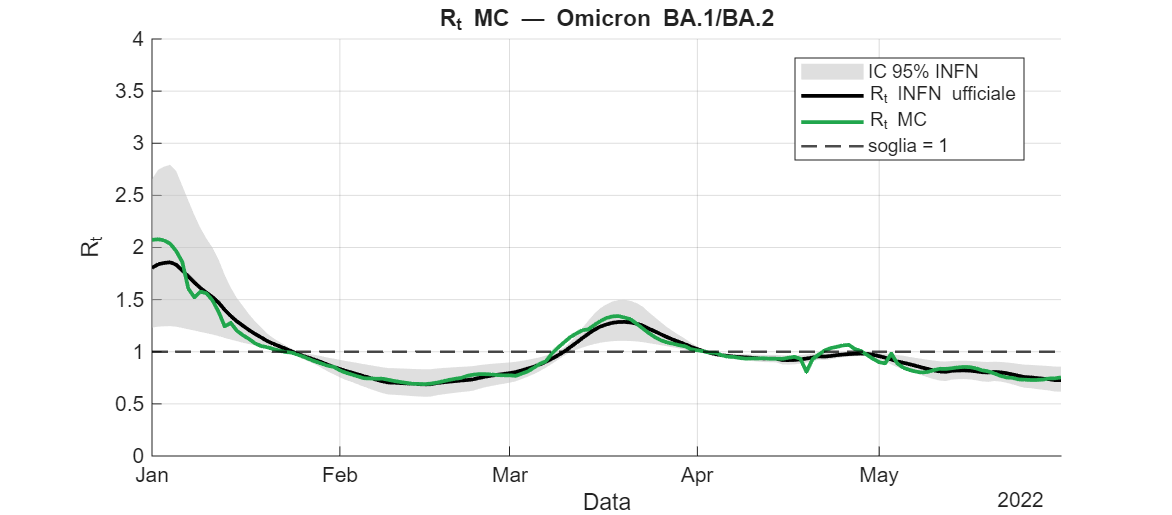
\includegraphics[width=\textwidth]{rt_mc_fase_3_Omicron_BA.1_BA.2.png}
        \caption{Fase 3 -- BA.1/BA.2.}
        \label{fig:mc_fase3}
    \end{subfigure}

    \vspace{0.5em}

    \begin{subfigure}[b]{0.48\textwidth}
        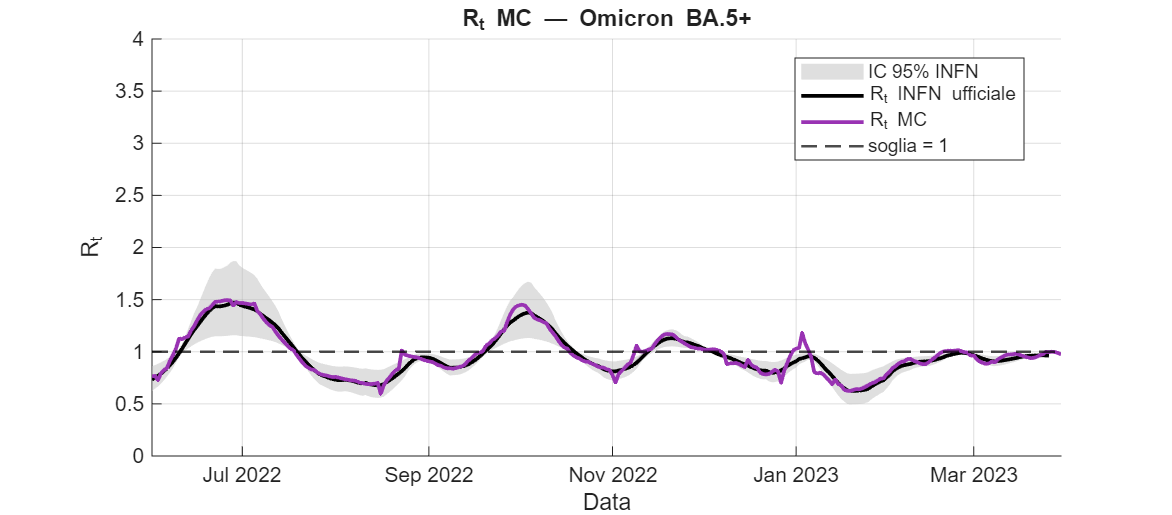
\includegraphics[width=\textwidth]{rt_mc_fase_4_Omicron_BA.5+.png}
        \caption{Fase 4 -- BA.5+.}
        \label{fig:mc_fase4}
    \end{subfigure}
    \hfill
    \begin{subfigure}[b]{0.48\textwidth}
        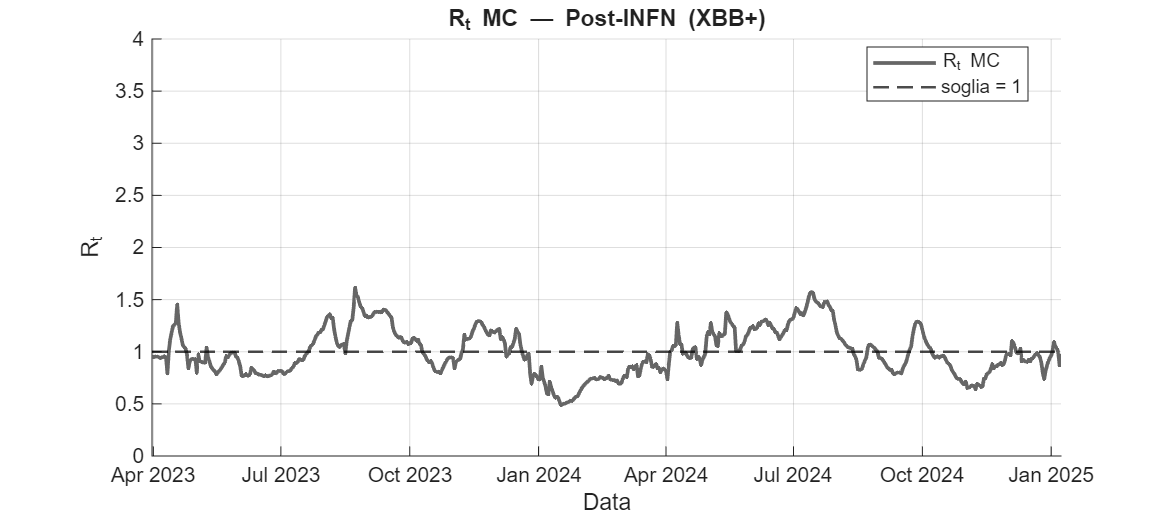
\includegraphics[width=\textwidth]{rt_mc_fase_5_Post-INFN_(XBB+).png}
        \caption{Fase 5 -- XBB+ (nessun dato INFN).}
        \label{fig:mc_fase5}
    \end{subfigure}
    \caption{Fasi 2--5, metodo MC Metropolis. Curva MC colorata, INFN ufficiale in nero,
             IC~95\% in grigio.}
    \label{fig:mc_fasi2-5}
\end{figure}

\begin{figure}[htbp]
    \centering
    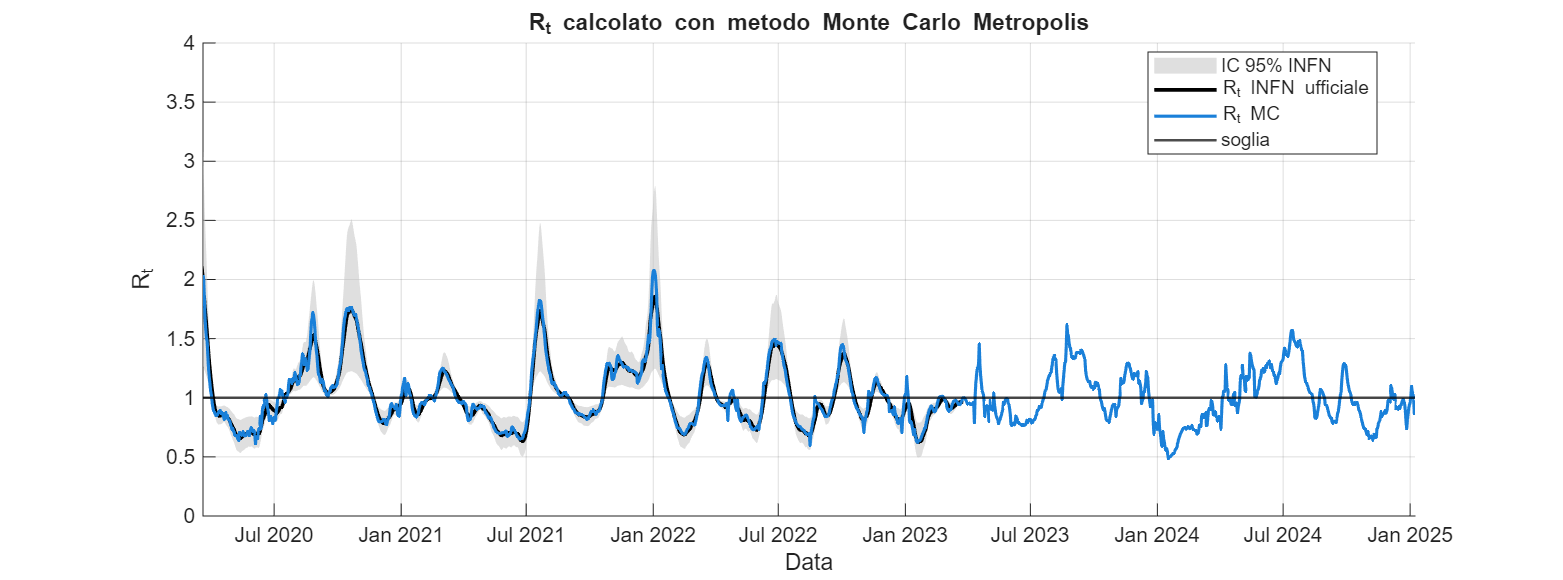
\includegraphics[width=\textwidth]{rt_mc_tutte_le_fasi.png}
    \caption{$R_t$ calcolato con il metodo MC su tutte le fasi.
             In blu la curva MC; in nero la curva INFN ufficiale con banda IC~95\% (grigio).}
    \label{fig:mc_all}
\end{figure}

La Tabella~\ref{tab:errori_mc} riassume l'errore massimo rispetto alla curva INFN
centrale per le fasi con dato di riferimento disponibile.

\begin{table}[htbp]
\centering
\caption{Errori metodo MC vs INFN per fase.}
\label{tab:errori_mc}
\begin{tabular}{llc}
\toprule
\textbf{Fase} & \textbf{Variante} & \textbf{Max $|R_t^{\text{MC}} - R_t^{\text{INFN}}|$} \\
\midrule
1 & Ancestrale + Alpha & 0{,}201 \\
2 & Delta              & 0{,}251 \\
3 & Omicron BA.1/BA.2  & 0{,}269 \\
4 & Omicron BA.5+      & 0{,}242 \\
\bottomrule
\end{tabular}
\end{table}

\noindent
La curva MC mostra un leggero \emph{anticipo} di circa una settimana rispetto al dato INFN
ufficiale: quest'ultimo viene pubblicato con un ritardo che incorpora correzioni retroattive
dei sintomatici, mentre il metodo MC calcola $R_t$ in modo causale su dati storici completi.
L'aumento dell'errore nelle fasi Omicron è atteso: i parametri $\varphi(s)$ sono stimati
sulla variante ancestrale~\cite{Guzzetta2020} e non vengono ricalibrati per le varianti
successive, il cui tempo di generazione più breve introduce una sistematicità nella stima.


% -------------------------------------------------------
\section{Stabilità di \texorpdfstring{$R_t$}{Rt} e confronto tra i metodi}
\label{sec:stabilita}
% -------------------------------------------------------

Un aspetto rilevante per l'uso operativo di $R_t$ è la \emph{stabilità temporale} della stima:
quanto cambia il valore calcolato per un giorno fissato $t_0$ all'aumentare dei dati disponibili?

\paragraph{Metodo SIR.}
La formula~\eqref{eq:rt_dpc} usa solo i dati locali al giorno $t_0$: $R_t(t_0)$ non viene
ricalcolato all'arrivo di nuovi dati successivi.
La stima è stabile entro pochi giorni dall'evento.
Il ritardo strutturale rispetto al dato ufficiale INFN (circa una settimana) è dovuto
all'uso di date di prelievo/referto in luogo della data di inizio sintomi.

\paragraph{Metodo Monte Carlo.}
Nell'implementazione proposta il calcolo usa i dati DPC \texttt{nuovi\_positivi} a
consuntivo: $\lambda_{\text{base}}(t) = \sum_{s=1}^{25} \varphi_s\, C(t-s)$ dipende solo
dai casi \emph{passati} rispetto a $t$.
Il valore $R_t(t_0)$ è quindi determinato una volta sola e non subisce aggiornamenti
retroattivi; la variabilità MCMC tra esecuzioni indipendenti è dell'ordine di $10^{-3}$.
L'anticipo di circa una settimana rispetto al dato INFN ufficiale è attribuibile al ritardo
con cui INFN pubblica i propri valori, che incorpora correzioni retroattive dei sintomatici ISS.

\begin{table}[htbp]
\centering
\caption{Confronto sintetico tra i metodi implementati.}
\label{tab:confronto}
\begin{tabular}{p{3.8cm}p{5.5cm}p{5cm}}
\toprule
\textbf{Proprietà}           & \textbf{Metodo SIR}             & \textbf{Metodo Monte Carlo} \\
\midrule
Dato di input                & Nuovi pos.\ (ISS o DPC)         & Sintomatici (ISS) \\
Parametro chiave             & $T_R$ (per variante)            & $\varphi(s)$ (Gamma) \\
Errore tipico su $R_t$       & $0{,}2$--$0{,}6$ (vs INFN)      & $0{,}2$--$0{,}3$ (vs INFN) \\
Sfasamento vs INFN           & Ritardo $\sim$1 settimana       & Anticipo $\sim$1 settimana \\
Incertezza parametrica       & Banda $T_R \pm \Delta T_R$      & Dipende da $\varphi(s)$ \\
\bottomrule
\end{tabular}
\end{table}

% -------------------------------------------------------
\subsection{Correlazione con eventi socio-politici}
% -------------------------------------------------------

La Figura~\ref{fig:eventi} sovrappone la curva $R_t$ Monte Carlo all'intero periodo epidemico,
annotando i principali provvedimenti normativi e le transizioni di variante.
I picchi e i cali di $R_t$ risultano correlati in modo sistematico con gli interventi di
restrizione e riapertura: il lockdown nazionale del 9 marzo 2020, le successive riaperture
graduali e infine il cambio di regime con la variante Delta (luglio 2021) e con Omicron
(gennaio 2022) sono tutti leggibili come discontinuità nella curva.

\begin{figure}[htbp]
    \centering
    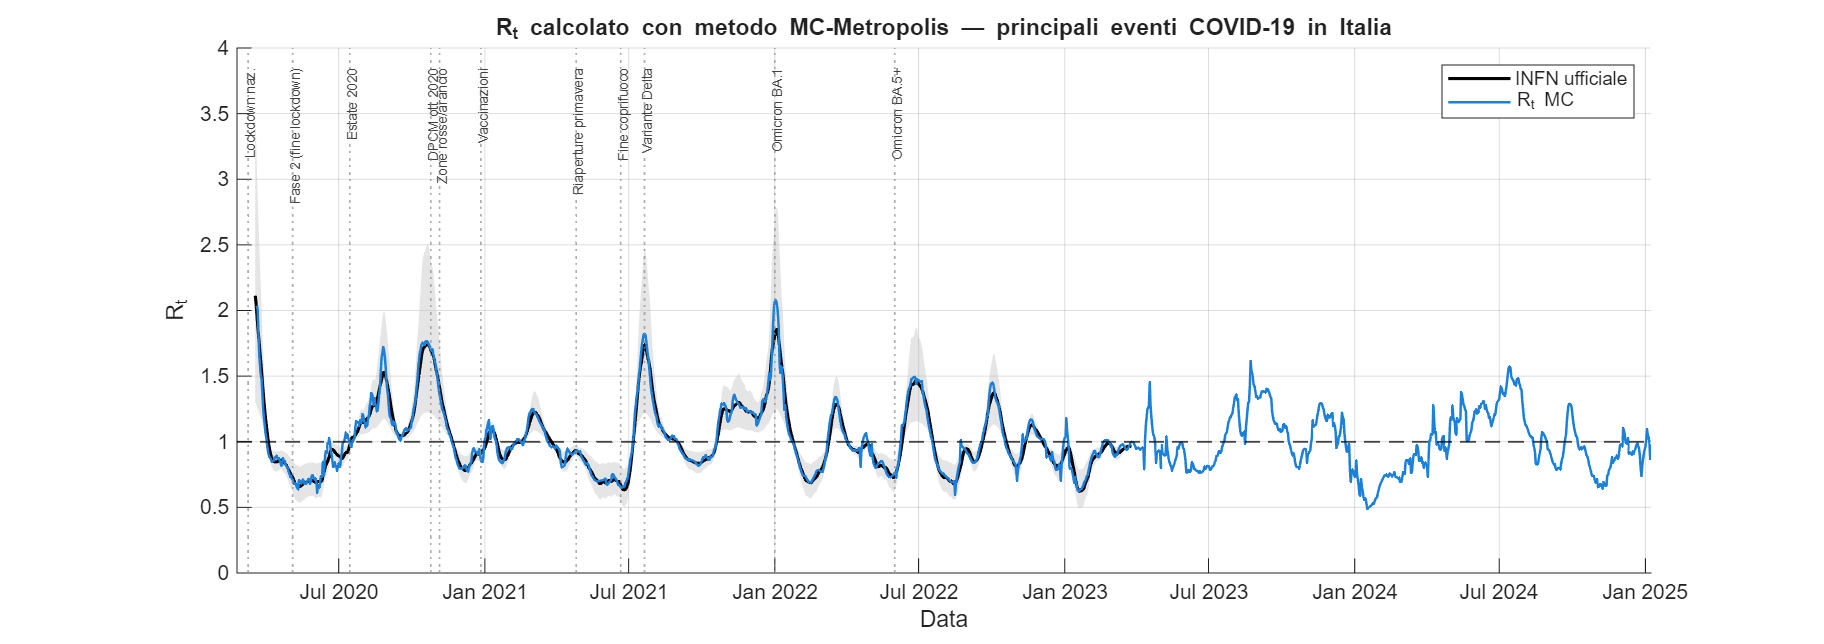
\includegraphics[width=\textwidth]{rt_mc_eventi.png}
    \caption{$R_t$ calcolato con il metodo Monte Carlo--Metropolis con annotazione dei
             principali eventi dell'epidemia in Italia.
             Le linee verticali tratteggiate indicano provvedimenti normativi e cambi di variante;
             la banda grigia è l'IC~95\% INFN.}
    \label{fig:eventi}
\end{figure}

% -------------------------------------------------------
\section{Conclusioni}
% -------------------------------------------------------

Sono stati implementati due metodi per il calcolo di $R_t$ sull'epidemia COVID-19 in Italia.

Il \textbf{metodo SIR} è semplice da implementare e interpretare, con un errore
che varia tra $0{,}2$ e $0{,}6$ rispetto al valore ufficiale INFN a seconda della fase.
La scelta del parametro $T_R$ è critica: usare il valore calibrato per l'ancestrale
($T_R = 9{,}7$ giorni) sulle varianti Omicron comporta una sovrastima sistematica
che cresce con $R_t$, poiché $R_t$ dipende linearmente da $T_R$, fino al 60\% ai picchi di ondata.
La visualizzazione delle bande $T_R \pm \Delta T_R$ quantifica esplicitamente questa
incertezza parametrica.

Il \textbf{metodo Monte Carlo--Metropolis} non dipende dal parametro $T_R$ ma sfrutta
la distribuzione dei tempi di generazione $\varphi(s)$ e la verosimiglianza poissoniana.
L'errore massimo rispetto a INFN varia tra $0{,}201$ (Fase~1) e $0{,}269$ (Fase~3),
sistematicamente inferiore al metodo SIR con sorgente DPC.
La curva MC mostra un leggero anticipo rispetto al dato INFN ufficiale, che incorpora
ritardi di pubblicazione e correzioni retroattive.

I due metodi sono complementari: il SIR è più diretto e richiede solo il dato degli attualmente
positivi; il Monte Carlo sfrutta la struttura temporale dei contagi ed è più accurato,
a costo di una maggiore complessità implementativa.

% -------------------------------------------------------
\begin{thebibliography}{9}

\bibitem{Lazzizzera2021}
I. Lazzizzera,
\textit{The SIR model towards the data: One year of Covid-19 pandemic in Italy case study
and plausible ``real'' numbers},
arXiv:2106.01602v2 [q-bio.PE], 2021.
\url{https://pmc.ncbi.nlm.nih.gov/articles/PMC8336674/}

\bibitem{Xu2023}
X. Xu, Y. Wu et al.,
\textit{Assessing changes in incubation period, serial interval, and generation time of
SARS-CoV-2 variants of concern: a systematic review and meta-analysis},
BMC Medicine, 21:375, 2023.
\url{https://doi.org/10.1186/s12916-023-03070-8}

\bibitem{Park2023}
S.\,W. Park et al.,
\textit{Inferring the differences in incubation-period and generation-interval distributions
of the Delta and Omicron variants of SARS-CoV-2},
PNAS, 120(22), e2221887120, 2023.
\url{https://doi.org/10.1073/pnas.2221887120}

\bibitem{Guzzetta2020}
G. Guzzetta, S. Merler,
\textit{Stime della trasmissibilità di SARS-CoV-2 in Italia},
Fondazione Bruno Kessler, Trento, 7 dicembre 2020.
\url{https://www.epicentro.iss.it/coronavirus/open-data/rt.pdf}

\bibitem{Merler2020}
S. Merler,
\textit{Monitoraggio di COVID-19 in Italia},
Fondazione Bruno Kessler / ISS, 2020.
\url{https://www.epicentro.iss.it/coronavirus/open-data/rt_diapo.pdf}


\bibitem{ISS_opendata}
Istituto Superiore di Sanità (ISS),
\textit{Dati Covid-19 -- casi per data di prelievo/diagnosi},
\url{https://www.epicentro.iss.it/coronavirus/sars-cov-2-sorveglianza-dati}.
File: \texttt{covid\_19-iss.xlsx}, foglio \texttt{casi\_prelievo\_diagnosi}.
Archivi storici per anno: \texttt{OPENDATA-\{anno\}.zip} dallo stesso dominio.

\bibitem{DPC_github}
Presidenza del Consiglio dei Ministri -- Dipartimento della Protezione Civile,
\textit{COVID-19 Italia -- Andamento nazionale},
GitHub, \url{https://github.com/pcm-dpc/COVID-19},
file \texttt{dati-json/dpc-covid19-ita-andamento-nazionale.json}.

\bibitem{INFN_rt}
INFN CovidStat,
\textit{Indice $R_t$ -- dati ufficiali CovidStat},
\url{https://covid19.infn.it/sommario/rt.html}
(dati estratti dal grafico interattivo, copertura 18~mar~2020 -- 30~mar~2023).

\bibitem{INFN_rt_info}
INFN CovidStat,
\textit{Metodologia per il calcolo di $R_t$},
\url{https://covid19.infn.it/sommario/rt-info.html}.

\bibitem{Cori2013}
A. Cori, N.\,M. Ferguson, C. Fraser, S. Cauchemez,
\textit{A New Framework and Software to Estimate Time-Varying Reproduction Numbers
During Epidemics},
American Journal of Epidemiology, 178(9):1505--1512, 2013.
\url{https://doi.org/10.1093/aje/kwt133}

\bibitem{Cereda2020}
D. Cereda et al.,
\textit{The early phase of the COVID-19 outbreak in Lombardy, Italy},
arXiv:2003.09320, 2020.
\url{https://arxiv.org/abs/2003.09320}

\bibitem{UKHSA2024}
UK Health Security Agency (UKHSA),
\textit{COVID-19: infectious period, asymptomatic and symptomatic transmission},
rapid evidence review (aggiornato settembre 2023).
\url{https://www.gov.uk/government/publications/covid-19-infectious-period-asymptomatic-and-symptomatic-transmission}

\bibitem{Keske2023}
\c{S}. Keske et al.,
\textit{Duration of infectious shedding of SARS-CoV-2 Omicron variant and its relation
with symptoms},
Clinical Microbiology and Infection, 29:221--224, 2023.
\url{https://doi.org/10.1016/j.cmi.2022.07.009}

\end{thebibliography}

\end{document}
